\documentclass{beamer}

\usetheme{Madrid}

\title[Projet compilation]{Projet compilation}
\author[Hexanomnom]{Théo Choné, Ewan Chorynski, Clément Giraudon \\ Zyad Haddad, Noham Martin, Clément Vial}
\institute[INSA Lyon]{INSA Lyon}
\date{2024}
\logo{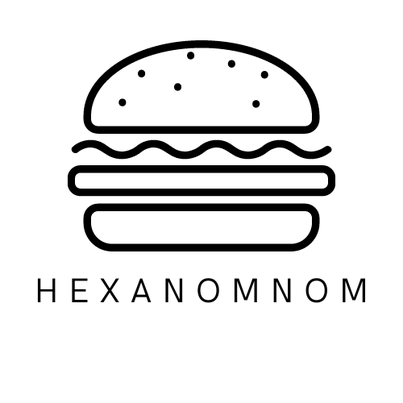
\includegraphics[width=1cm]{logo.png}}

\usepackage[T1]{fontenc}
\usepackage[utf8]{inputenc}
\usepackage{listings}
\usepackage{tikz}
\usepackage{xcolor}
\usetikzlibrary{positioning}
\usetikzlibrary{shapes.geometric}

\lstset{%
basicstyle=\ttfamily,
breaklines = true,
language=C,
numbers=left,
numberstyle=\tiny\color{gray},
keywordstyle=\color{blue}\ttfamily,
stringstyle=\color{red}\ttfamily,
commentstyle=\color{green}\ttfamily,
morecomment=[l][\color{magenta}]{\#},
xleftmargin=2em,frame=single,framexleftmargin=1.5em
}

\newcommand*{\thead}[1]{\multicolumn{1}{|c|}{\bfseries #1}}
\newcommand*{\local}[1]{\lstinline|\_#1|}

\begin{document}

\frame{\titlepage}

\begin{frame}
    \frametitle{Table des matières}
    \tableofcontents
\end{frame}

\section{Fonctionnalités implémentées}

\begin{frame}
    \frametitle{Fonctionnalités implémentées}
    \framesubtitle{Fonctionnalités obligatoires}
    \begin{center}
        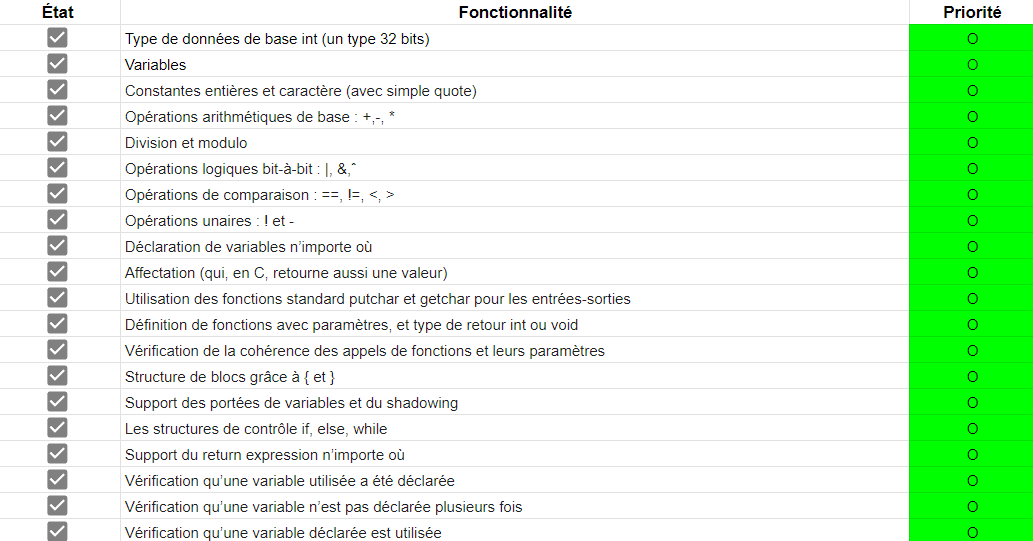
\includegraphics[width=\textwidth,height=0.8\textheight,keepaspectratio]{fonctionnalite1.png}
    \end{center}
\end{frame}

\begin{frame}
    \frametitle{Fonctionnalités implémentées}
    \framesubtitle{Fonctionnalités facultatives}
    \begin{center}
        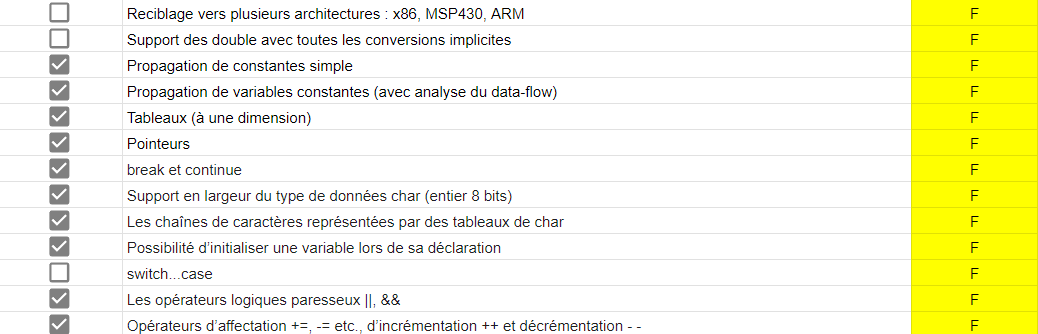
\includegraphics[width=\textwidth,height=0.8\textheight,keepaspectratio]{fonctionnalite2.png}
    \end{center}
\end{frame}

\begin{frame}
    \frametitle{Fonctionnalités implémentées}
    \framesubtitle{Fonctionnalités bonus}
    \begin{center}
        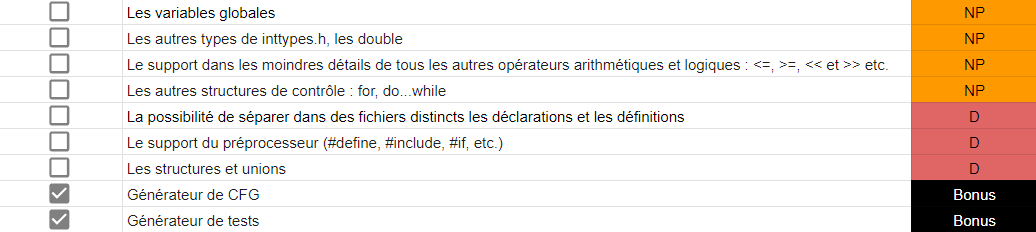
\includegraphics[width=\textwidth,height=0.8\textheight,keepaspectratio]{fonctionnalite3.png}
    \end{center}
\end{frame}

\section{Représentation intermédiaire}

\begin{frame}
    \frametitle{Représentation intermédiaire}
    \framesubtitle{La structure}

    \begin{block}{Control flow graph}
        \begin{itemize}
            \item Classe \lstinline{Function} (\lstinline{ir/Function.h})
            \item Liste de \lstinline{BasicBlock} 
            \item Blocs spéciaux : prologue et épilogues
            \item Informations propres à une fonction
        \end{itemize}
    \end{block}
    \pause
    \begin{block}{Bloc basique}
        \begin{itemize}
            \item Classe \lstinline{BasicBlock} (\lstinline{ir/BasicBlock.h})
            \item Liste d'\lstinline{Instruction} 
            \item Un \lstinline{Terminator}
        \end{itemize}
    \end{block}
\end{frame}

\begin{frame}
    \frametitle{Représentation intermédiaire}
    \framesubtitle{Les opérandes}
    \begin{block}{Variable locale}
        \begin{itemize}
            \item Classe \lstinline{Local}
            \item Possède un type
            \item Simplement un ID, noté \local{i}
            \item La variable locale \local{0} stocke la valeur de retour
            \item Les variables suivantes stockent d'abord les arguments (\local{1} est le premier argument)
        \end{itemize}
    \end{block}
    \pause
    \begin{block}{Les constantes (ou immédiates)}
        \begin{itemize}
            \item Classe \lstinline{Immediate}
            \item Possède un type
            \item Simplement un nombre connu à la compilation
        \end{itemize}
    \end{block}
\end{frame}

\begin{frame}
    \frametitle{Représentation intermédiaire}
    \framesubtitle{Les opérandes}

    \begin{block}{RValues}
        \begin{itemize}
            \item Alias \lstinline{RValue}
            \item Représente soit une \lstinline{Local} soit une \lstinline{Immediate}
            \item Utilise \lstinline{std::variant}
        \end{itemize}
    \end{block}
    \pause
    \begin{block}{Les chaînes de caractères litérales}
        \begin{itemize}
            \item Classe \lstinline{StringLiteral}
            \item Représente une chaîne de caractères qui sera dans l'exécutable
        \end{itemize}
    \end{block}
    \pause
    \begin{block}{Les éléments dont on peut prendre l'adresse}
        \begin{itemize}
            \item Classe \lstinline{Addressable}
            \item Représente soit une \lstinline{Local} soit une \lstinline{StringLiteral}
            \item Utilise \lstinline{std::variant}
        \end{itemize}
        
    \end{block}

\end{frame}

\begin{frame}
    \frametitle{Représentation intermédiaire}
    \framesubtitle{Les instructions}
    \begin{itemize}
        \item Descendants de la classe \lstinline{Instruction} (\lstinline{ir/Instructions.h})
        \item Instruction simple $\leftrightarrow$ pas de saut
    \end{itemize}
    \pause
    \begin{center}
        \begin{tabular}{ | l | l | l | }
        \hline
        \thead{Classe} & \thead{Notation} & \thead{Description} \\
        \hline 
        Assignment & local := rvalue & Simple assignation \pause \\ 
        \hline 
        UnaryOp & local := op rvalue & Opération unaire \pause \\
        \hline
        BinaryOp & local := rvalue op rvalue & Opération binaire \pause \\
        \hline
        Call & local := f(rvalue, ...) & Appel de fonction \pause \\
        \hline
        Cast & local := (type) rvalue & Changement de taille \pause \\
        \hline
        PointerRead & local := *rvalue & Lecture de pointeur \pause \\
        \hline
        PointerWrite & *rvalue := rvalue & Écriture de pointeur \pause \\
        \hline
        AddressOf & local := \&addressable & Stockage d'une adresse\\
        \hline
        \end{tabular}
    \end{center}
\end{frame}

\begin{frame}
    \frametitle{Représentation intermédiaire}
    \framesubtitle{Les instructions terminales}
    \begin{itemize}
        \item Descendants de la classe \lstinline{Terminator} (\lstinline{ir/Terminators.h})
        \item Instructions de saut pour terminer un bloc
    \end{itemize}
    \pause
    \begin{block}{Saut basique}
        \begin{itemize}
            \item Classe \lstinline{BasicJump}
            \item Un seul bloc de destination
        \end{itemize}
    \end{block}
    \pause
    \begin{block}{Saut conditionel}
        \begin{itemize}
            \item Classe \lstinline{ConditionalJump}
            \item Deux blocs de destination
            \item Une \lstinline{RValue} qui est la condition
        \end{itemize}
    \end{block}
\end{frame}
\begin{frame}[fragile]
    \frametitle{Exemple de représentation intermédiaire}

    \begin{columns}
        \begin{column}{.5\textwidth}
            \onslide<2->
            \begin{center}
                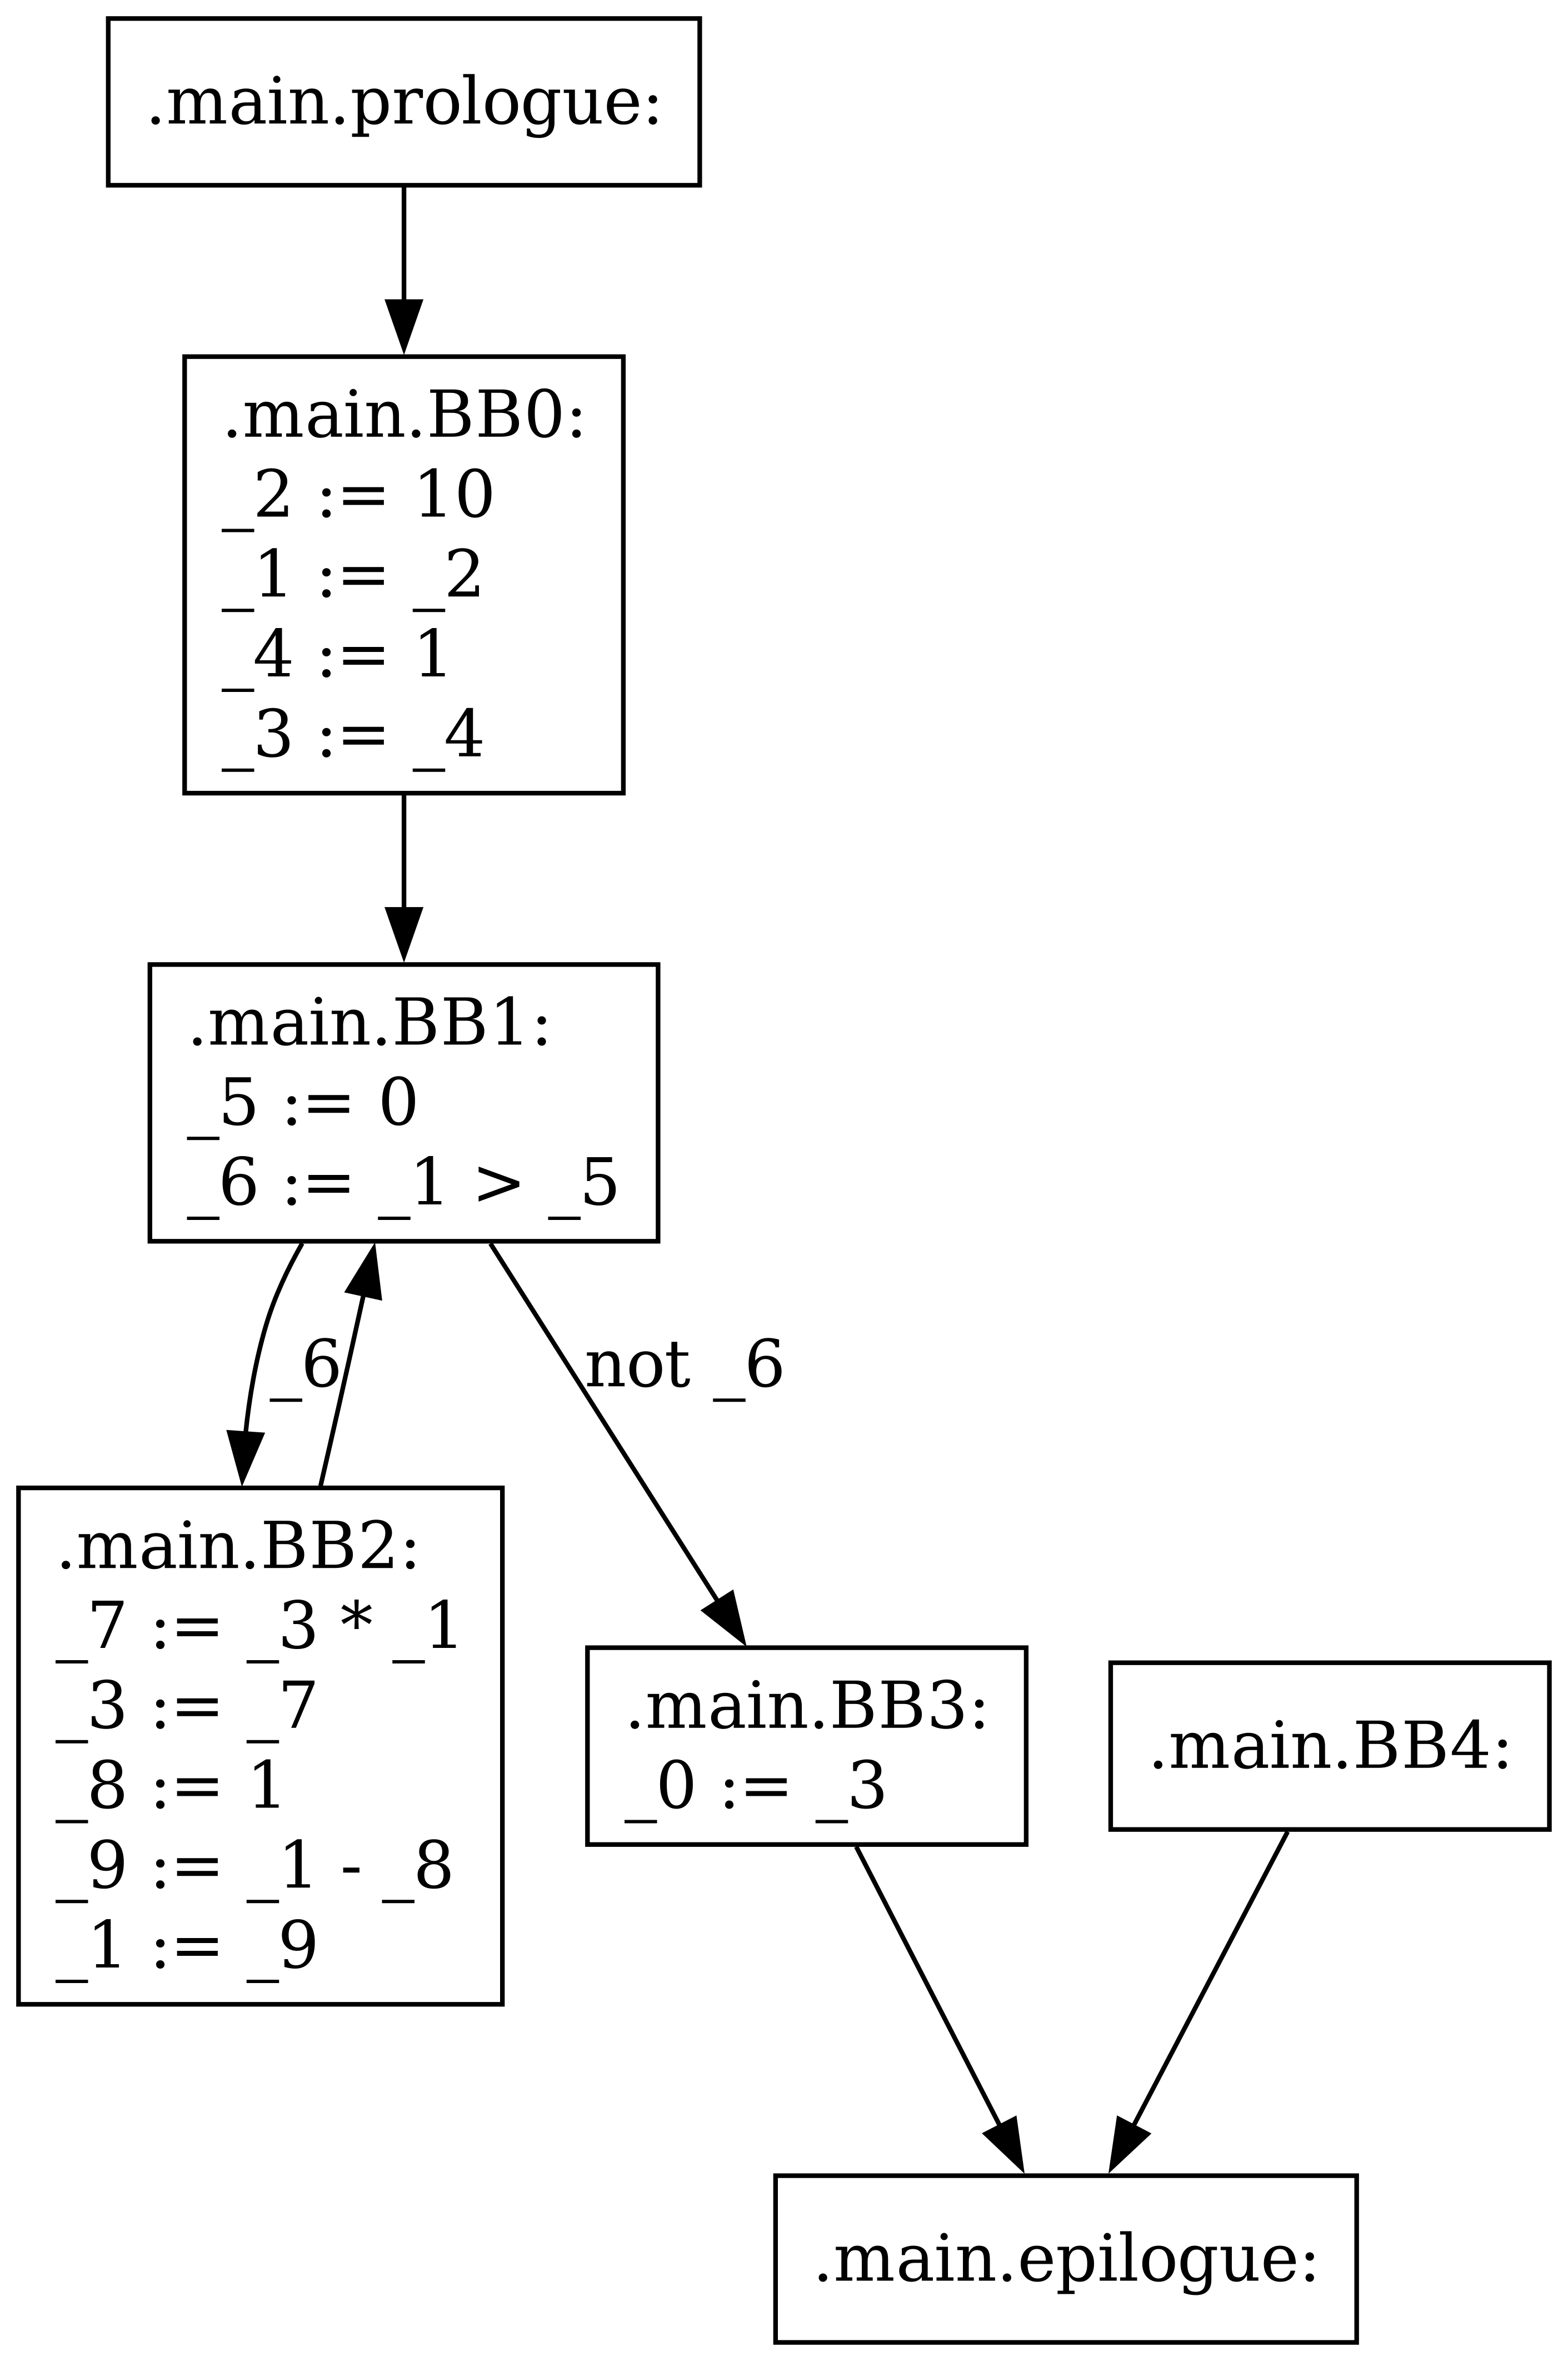
\includegraphics[width=\textwidth,height=0.8\textheight,keepaspectratio]{graphs/fact_no_opti.dot.png}
            \end{center}
        \end{column}
        \begin{column}{.5\textwidth}
            \onslide<1->
            \begin{lstlisting}
int main(){
    int x = 10;
    int y = 1;
    while(x > 0){
        y = y * x;
        x = x - 1;
    }
    return y;
}
            \end{lstlisting}
            La génération de graphe se fait à l'aide de la classe /lstinline{IrGraphVisitor.h}
        \end{column}
    \end{columns}

\end{frame}
\begin{frame}
    \frametitle{Visite de l'IR}
    \framesubtitle{Parcours}
    \begin{block}{Design pattern Visiteur}
        \begin{itemize}
            \item On utilise le design pattern Visiteur pour parcourir notre IR 
            \item Utilisation de la classe Visitor (\lstinline{ir/Visitor.h})
            \item Les classes \lstinline{Function}, \lstinline{BasicBlock}, \lstinline{Instructions} et \lstinline{Terminators} implémentent tous l'interface Visitable (\lstinline{ir/Visitable.h})
        \end{itemize}
    \end{block}
\end{frame}

\section{Optimisations sur l'IR}

\begin{frame}
    \frametitle{La pipeline}
    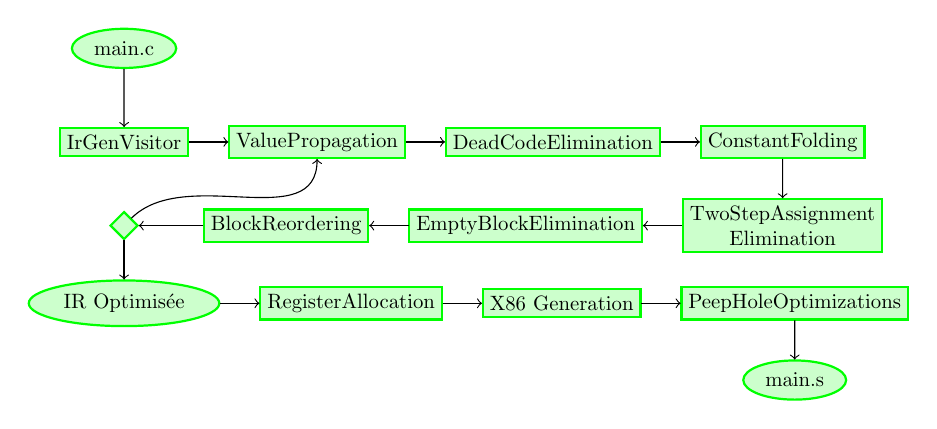
\begin{tikzpicture}[node distance={5mm}, main/.style = {draw=green!200, fill=green!20, thick, 
        rectangle, scale=0.75, align=center}]
        \node[main, ellipse] (1) {main.c};
        \node [main] (2)  [below=1] {IrGenVisitor};
        \draw[->] (1) -- (2);
        \node [main] (3) [right=of 2] {ValuePropagation};
        \draw[->] (2) -- (3);
        \node [main] (4) [right=of 3] {DeadCodeElimination};
        \draw[->] (3) -- (4);
        \node [main] (5) [right=of 4] {ConstantFolding};
        \draw[->] (4) -- (5);
        \node [main] (6) [below=of 5] {TwoStepAssignment \\ Elimination};
        \draw[->] (5) -- (6);
        \node [main] (7) [left=of 6] {EmptyBlockElimination};
        \draw[->] (6) -- (7);
        \node [main] (8) [left=of 7] {BlockReordering};
        \draw[->] (7) -- (8);
        \node [main, diamond, aspect=1] (9) at (2 |- 8) {};
        \draw[->] (9) to [in=-90] (3);
        \draw[->] (8) -- (9);
        \node[main, ellipse] (10) [below=of 9]{IR Optimisée};
        \draw[->] (9) -- (10);
        \node [main] (11) [right=of 10] {RegisterAllocation};
        \draw[->] (10) -- (11);
        \node [main] (12) [right=of 11] {X86 Generation};
        \draw[->] (11) -- (12);
        \node [main] (13) [right=of 12] {PeepHoleOptimizations};
        \draw[->] (12) -- (13);
        \node[main, ellipse] (14) [below=of 13]{main.s};
        \draw[->] (13) -- (14);
        \onslide<1->
    \end{tikzpicture}
\end{frame}

\begin{frame}[fragile]
    \frametitle{Propagation de variables et de constantes}
    \framesubtitle{Version simple}

    \begin{block}{Principe}
        Si on a une instruction d'assignation de la forme \lstinline{a := b}, remplacer
        toutes les utilisations de \lstinline{a} par des utilisations de \lstinline{b}
    \end{block}
    \pause
    \begin{exampleblock}{Exemple}
         \begin{columns}
            \begin{column}{.40\textwidth}
                    \begin{lstlisting}
_1 := 5
_2 := _1
_3 := _6
_4 := _3
_5 := _2 + _3
                    \end{lstlisting}
            \end{column}
            \pause
            \begin{column}{.04\textwidth}
                $\rightarrow$
            \end{column}
            \begin{column}{.40\textwidth}
                    \begin{lstlisting}
_1 := 5
_2 := 5
_3 := _6
_4 := _6
_5 := 5 + _6
                    \end{lstlisting}
            \end{column}
        \end{columns}       
    \end{exampleblock}
\end{frame}
\begin{frame}
    \frametitle{Propagation de variables et constantes}
    \framesubtitle{Version analyse du dataflow}

    \begin{block}{Limite de la version simple}
        Connaissances limitées au sein d'un bloc $\rightarrow$ fonctionne beaucoup moins bien lorsqu'il y a des branches
    \end{block}
    \pause
    \begin{block}{Analyse du dataflow}
        On va calculer les variables connues à la fin de chaque bloc afin de les propager au bloc suivant (classe \lstinline{BlockLivenessAnalysis.h})
    \end{block}

    \pause
    \begin{alertblock}{Attention}
        Si un bloc a plusieurs parents qui ne sont pas d'accord sur la valeur d'une variable,
        alors on ne peut pas conclure sur la valeur de cette variable au début du bloc
    \end{alertblock}
    
\end{frame}

\begin{frame}
    \frametitle{Propagation de variables et constantes}
    \framesubtitle{Exemple}
    \lstinputlisting{graphs/ex_propagation.c}
\end{frame}

\begin{frame}
    \frametitle{Propagation de variables et constantes}
    \framesubtitle{Exemple}
         \begin{columns}
            \begin{column}{.40\textwidth}
                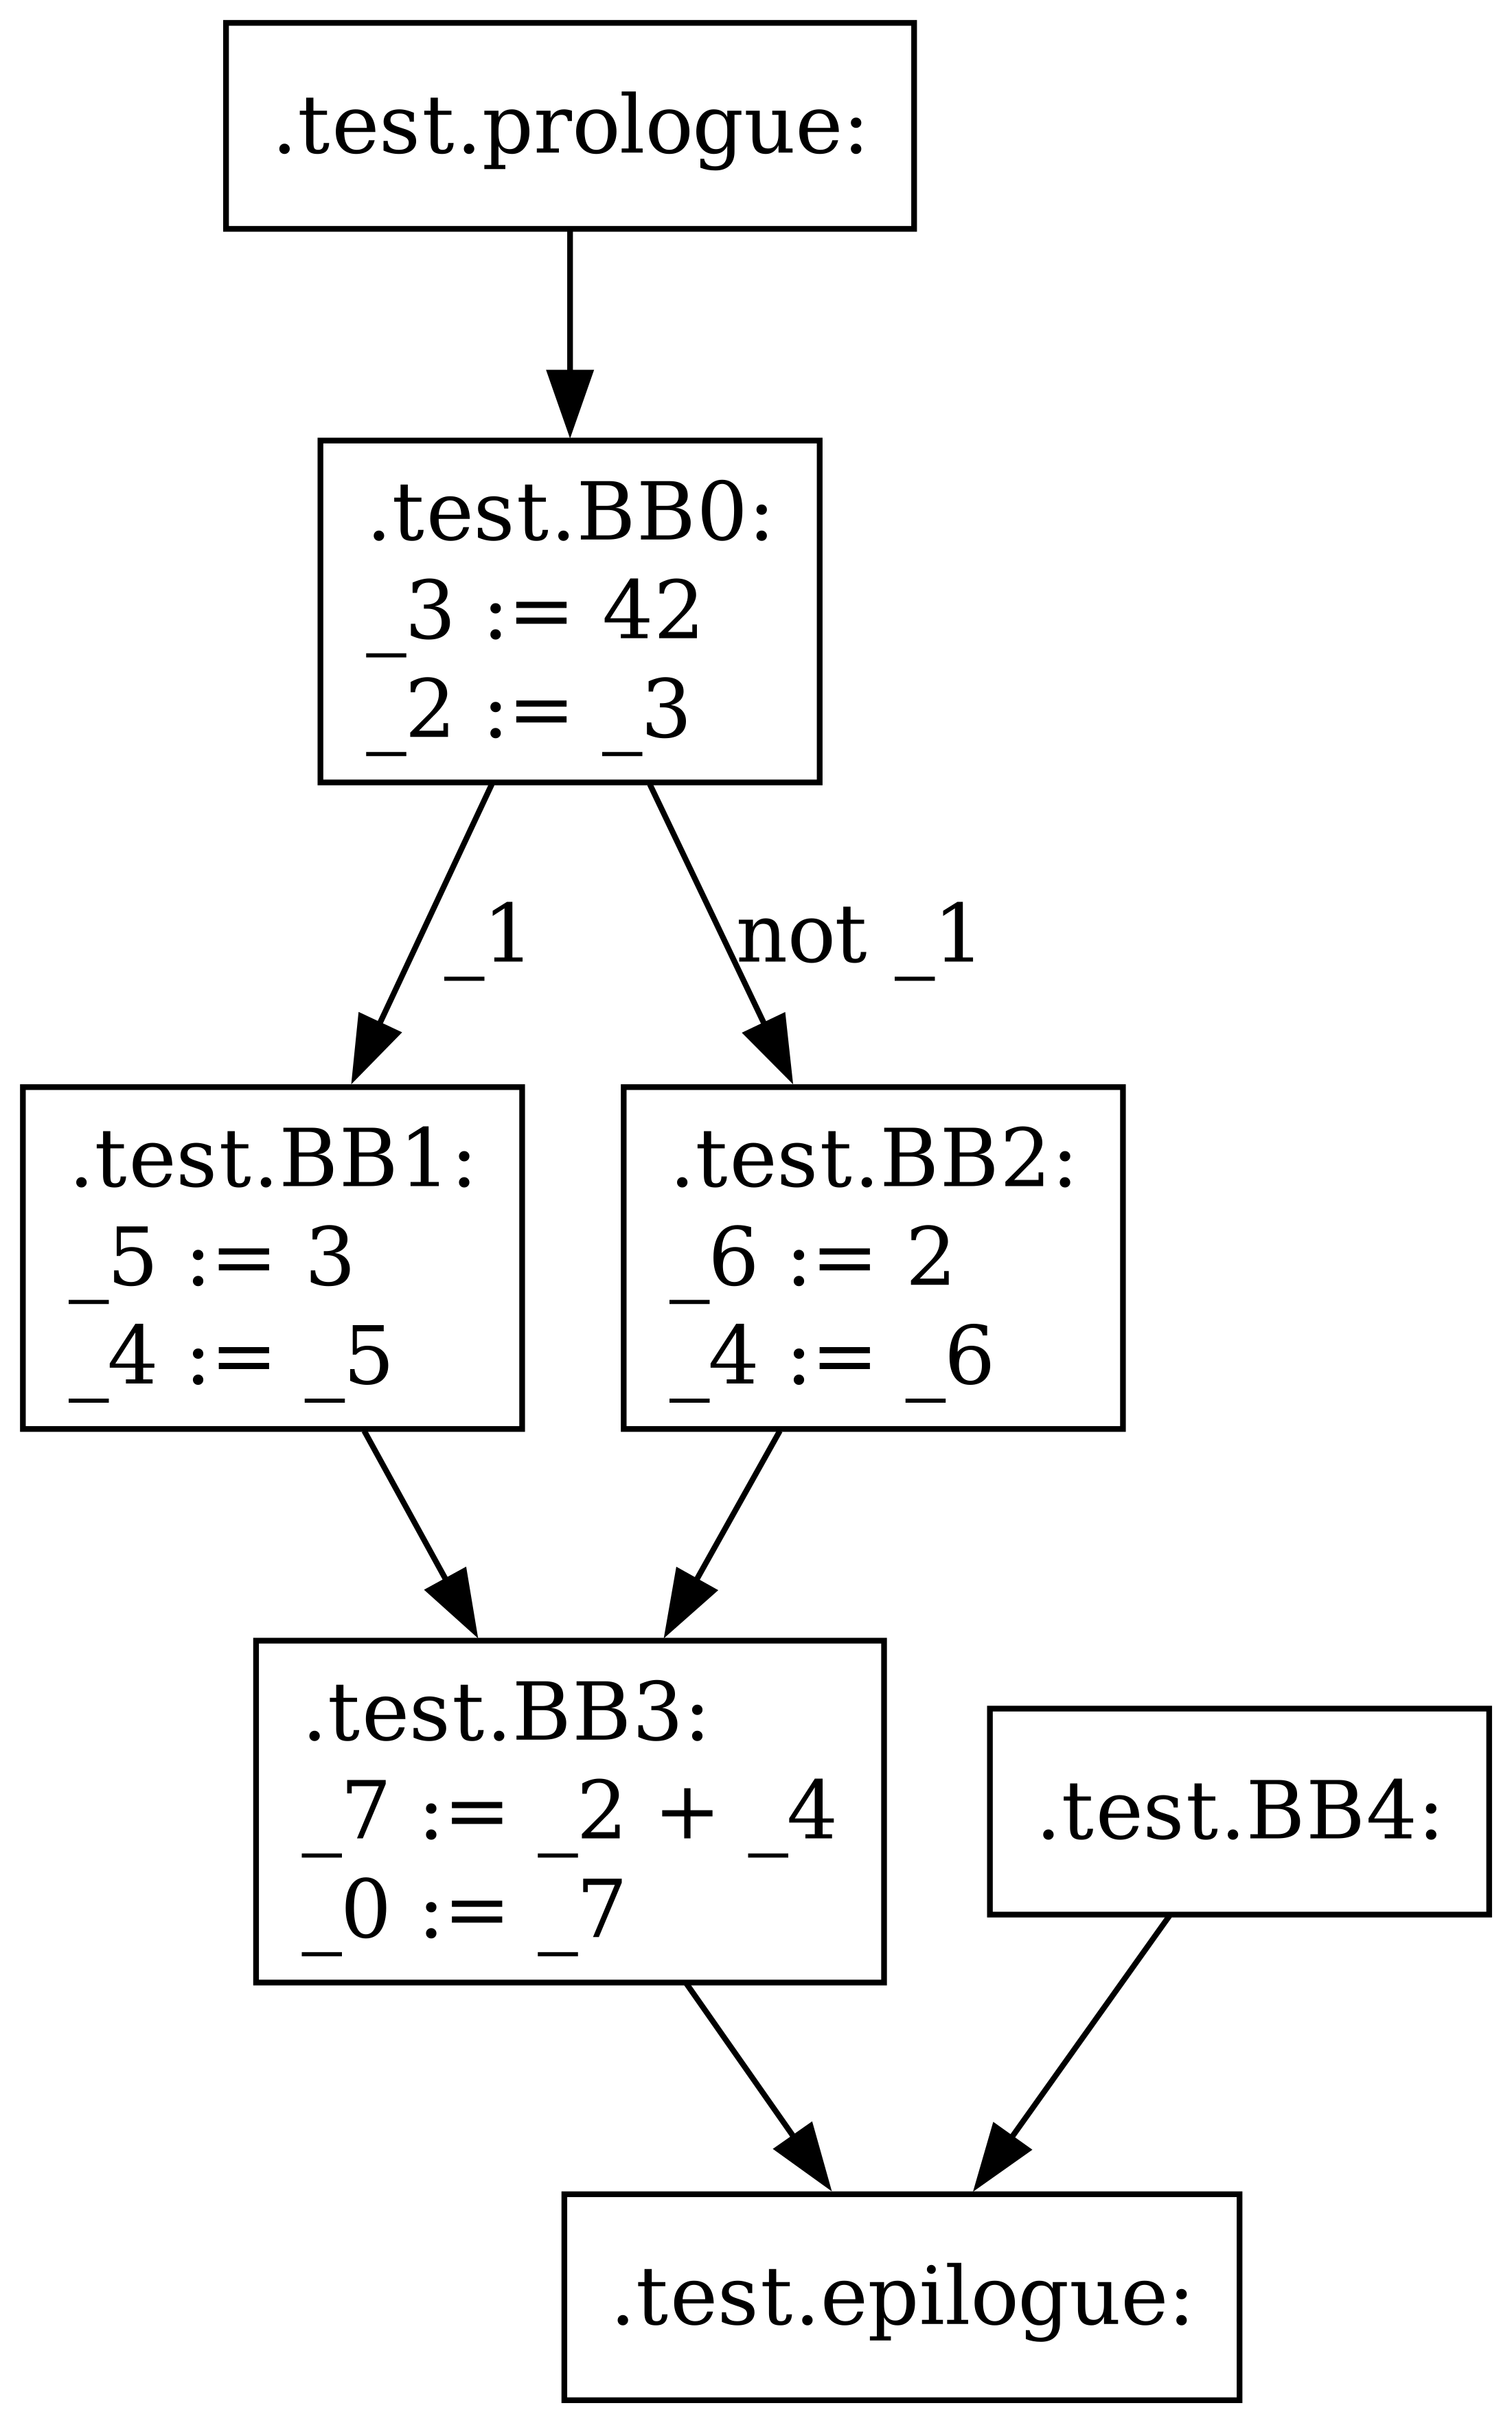
\includegraphics[width=\textwidth,height=0.8\textheight,keepaspectratio]{graphs/ex_propagation.dot.png}
            \end{column}
            \pause
            \begin{column}{.04\textwidth}
                $\rightarrow$
            \end{column}
            \begin{column}{.40\textwidth}
                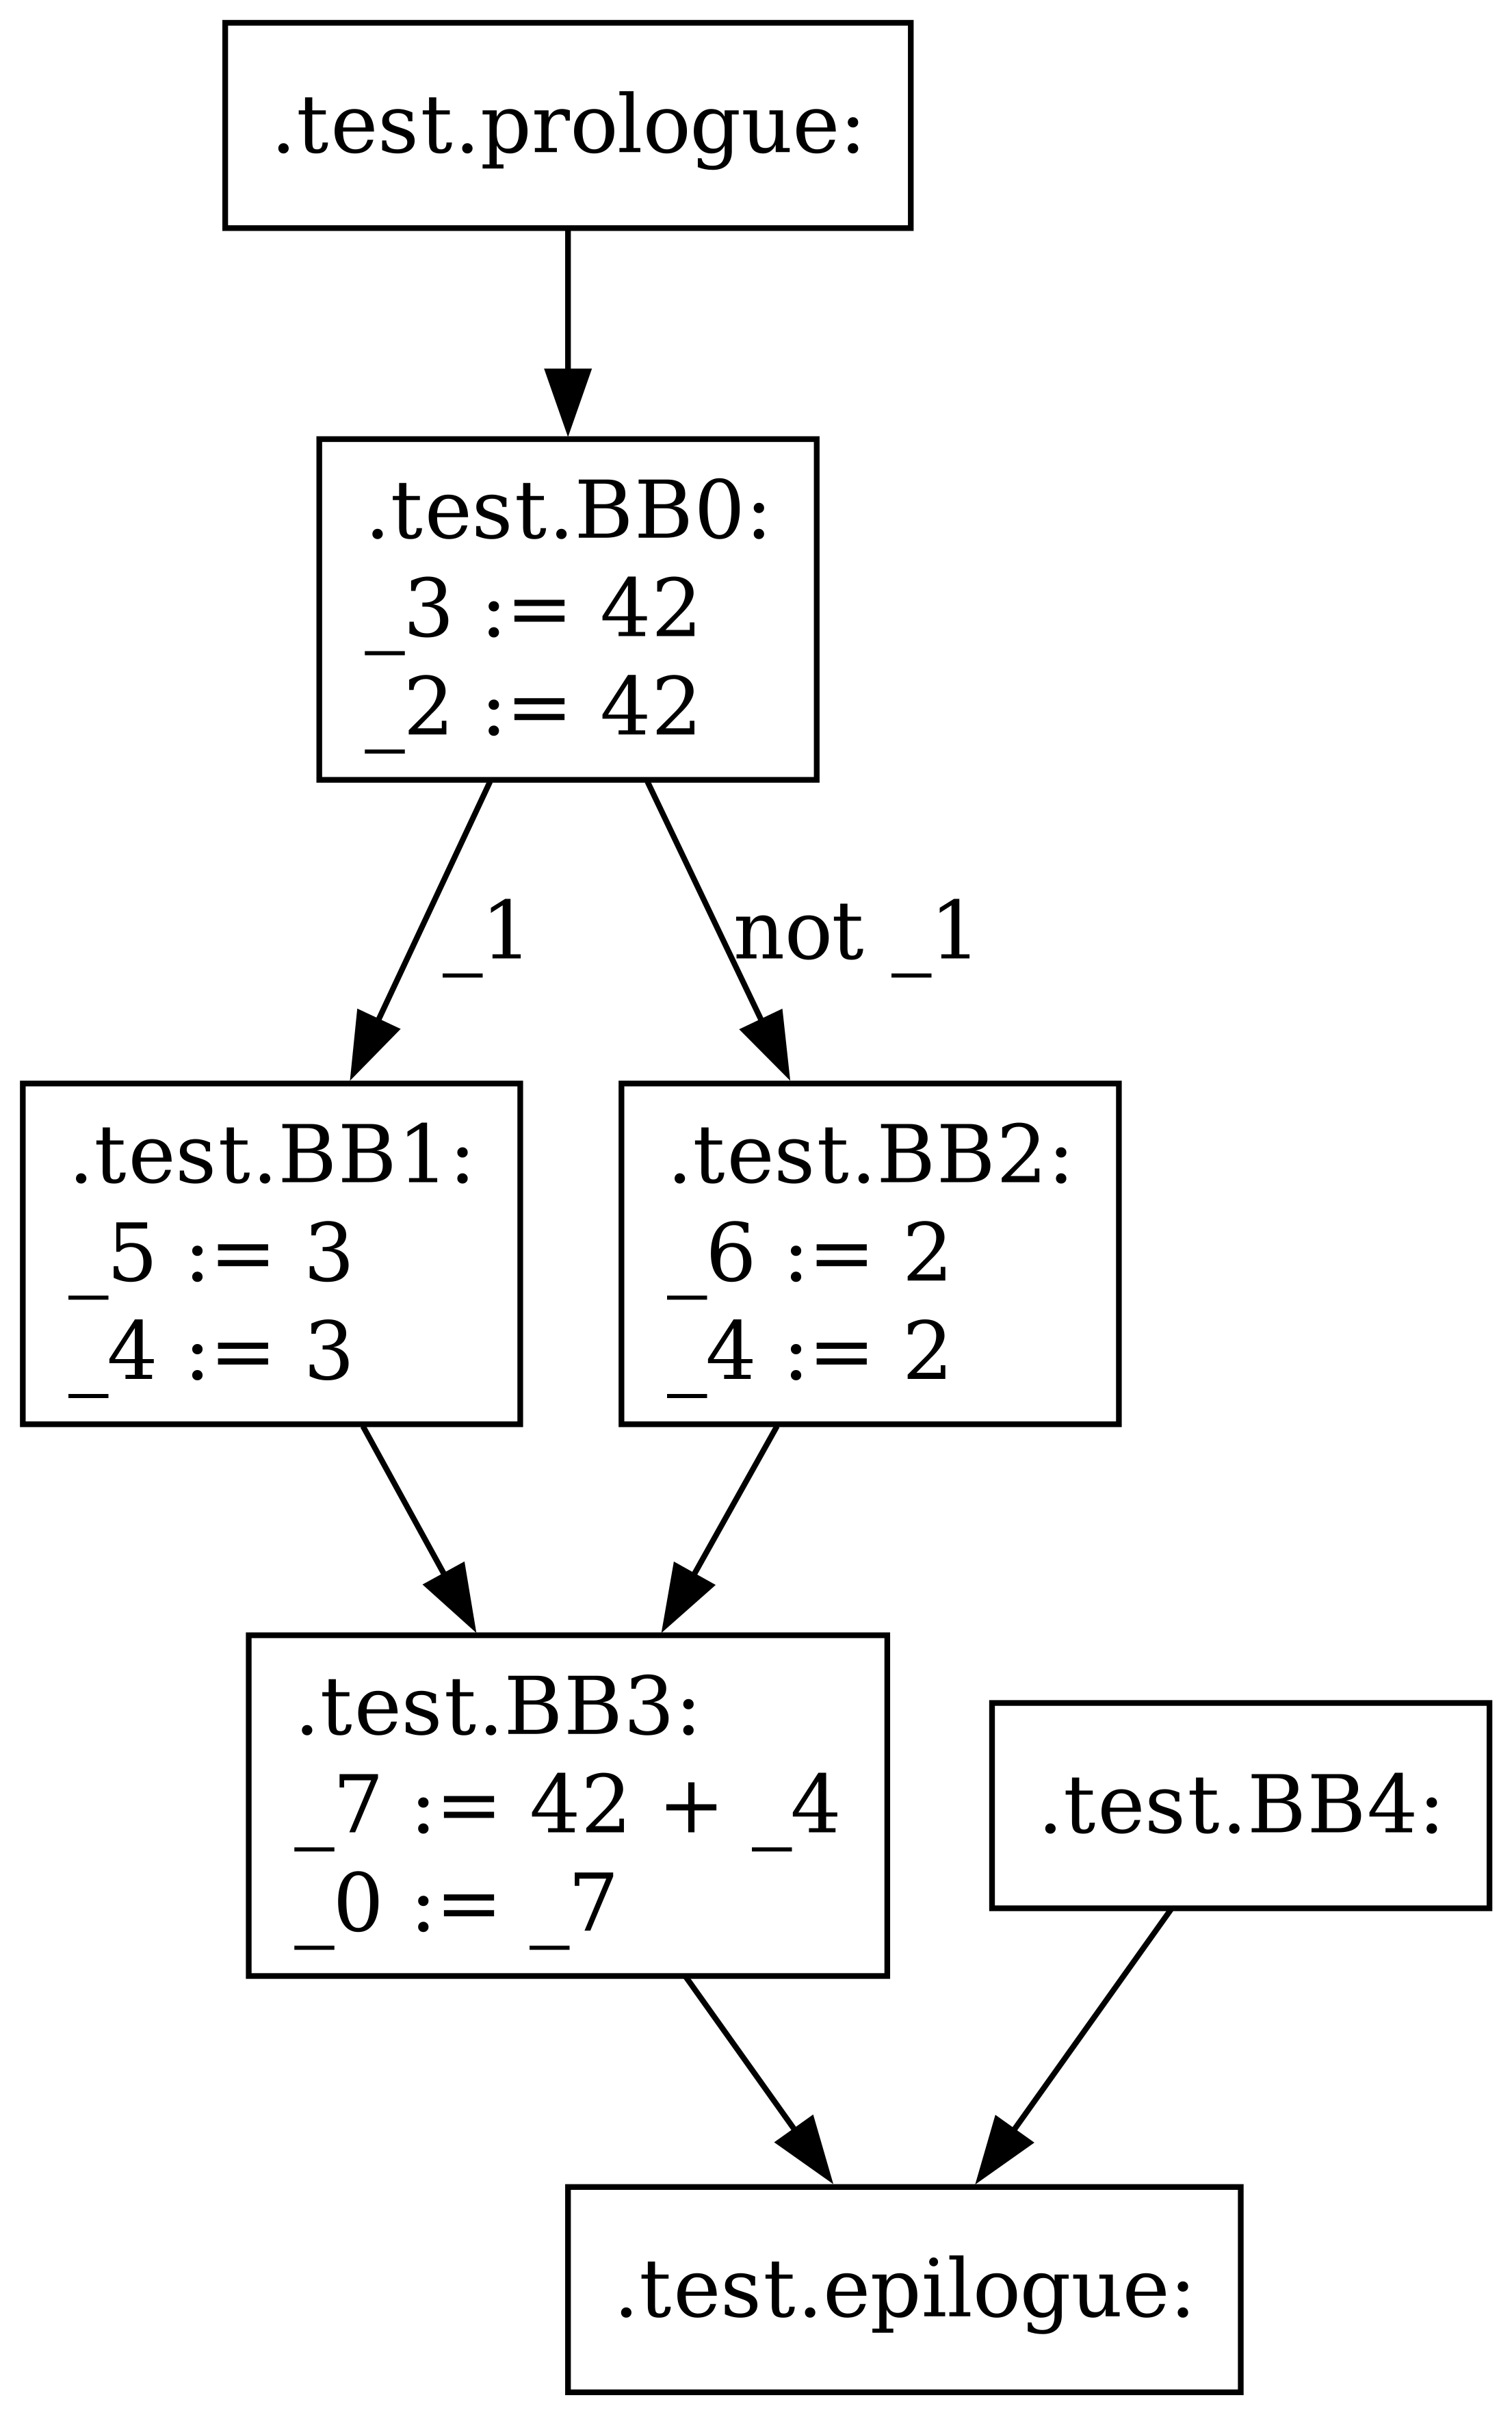
\includegraphics[width=\textwidth,height=0.8\textheight,keepaspectratio]{graphs/ex_propagation_after.dot.png}
            \end{column}
        \end{columns}       
\end{frame}

\begin{frame}[fragile]
    \frametitle{Élimination de code mort}
    \framesubtitle{Principe}
    
    \begin{block}{Principe}
        On sent bien qu'après la propagation, des variables assignées ne seront plus
        utilisées : on peut donc les éliminer. En pratique, on parcourt un bloc
        à l'envers (visiteur /lstinline{BlockDependance.h}) en marquant les variables 
        utilisées comme vivantes et les variables inutilisées comme mortes.

    \end{block}
    \pause
    \begin{exampleblock}{Exemple}
        Imaginons dans l'exemple précédent que seule \lstinline{_5} est utilisée par la suite
         \begin{columns}
            \begin{column}{.40\textwidth}
                    \begin{lstlisting}
_1 := 5
_2 := 5
_3 := _6
_4 := _6
_5 := 5 + _6
                    \end{lstlisting}
            \end{column}
            \pause
            \begin{column}{.04\textwidth}
                $\rightarrow$
            \end{column}
            \begin{column}{.40\textwidth}
                    \begin{lstlisting}
_5 := 5 + _6

                    \end{lstlisting}
            \end{column}
        \end{columns}       
    \end{exampleblock}
\end{frame}

\begin{frame}
    \frametitle{Élimination de code mort}
    \framesubtitle{Analyse de vivacité}
    \begin{alertblock}{Problème}
        Pour pouvoir affirmer au sein d'un bloc qu'une variable n'est pas utilisée,
        il faut connaître les variables utilisées par les blocs suivants. 
    \end{alertblock}
    \pause
    \begin{block}{Solution}
        Comme pour la propagation de constantes, on a besoin de propager les informations
        de vivacité d'un bloc au suivant. Notamment, un bloc propagera les variables
        vivantes en entrée vers l'ensemble des variables vivantes en sortie de ses
        prédécesseurs.
    \end{block}
    \pause
    \begin{block}{Remarque}
        En pratique, cette analyse est ensuite très utilisée dans tout le compilateur.
        Elle génère notamment le graphe d'interférence et collecte les variables qui doivent
        être préservées à travers les appels de fonction.
    \end{block}
\end{frame}

\begin{frame}[fragile]
    \frametitle{Calcul d'expression constante}
    \framesubtitle{Principe}

    \begin{block}{Principe}
        \begin{itemize}
            \item Si une instruction a toutes ses rvalues constantes, alors on peut calculer la valeur directement.
            \item Si un saut conditionel a une condition constante, alors on peut la remplacer
                  par un saut basique vers le bon bloc.
        \end{itemize}
    \end{block}
    \pause
    \begin{exampleblock}{Exemple}
         \begin{columns}
            \begin{column}{.40\textwidth}
                    \begin{lstlisting}
_1 := 5 + 3 
_2 := 5 - 2
_3 := 3 > 0
                    \end{lstlisting}
            \end{column}
            \pause
            \begin{column}{.04\textwidth}
                $\rightarrow$
            \end{column}
            \begin{column}{.40\textwidth}
                    \begin{lstlisting}
_1 := 8
_2 := 3
_3 := 1

                    \end{lstlisting}
            \end{column}
        \end{columns}       
    \end{exampleblock}
\end{frame}

\begin{frame}[fragile]
    \frametitle{Autres optimisations implémentées}
    \begin{block}{Optimisation d'assignation inutile}
        Si \local{1} n'est pas utilisée après la ligne 1 (sauf ligne 3) et que \local{2} 
        n'est pas utilisée entre la ligne 1 et 3 :
        \begin{columns}
            \begin{column}{.40\textwidth}
                    \begin{lstlisting}
_1 := anything
...
_2 := _1
                    \end{lstlisting}
            \end{column}

            \begin{column}{.04\textwidth}
                $\rightarrow$
            \end{column}
            \begin{column}{.40\textwidth}
                    \begin{lstlisting}
_2 := anything
...
                    \end{lstlisting}
            \end{column}
        \end{columns}
    \end{block}
    \pause
    \begin{block}{Optimisation des sauts}
        \begin{itemize}
            \item Si on jump vers un bloc vide $A$ qui fait seulement un jump basique $B$, alors on peut jump directement vers un bloc $B$ 
            \item Dans certaines conditions, on peut fusionner avec notre cible
            \item Autres optimisations de sauts conditionels quand la condition est la même
        \end{itemize}
    \end{block}
\end{frame}

\begin{frame}
    \frametitle{Autres optimisations implémentées}

    \begin{block}{Réorganisation des blocs}
        \begin{itemize}
            \item Parcours en profondeur du control flow graph et collecte des blocs parcourus
            \item Suppression des blocs inatteignables
            \item Idée de maximiser les jump directement vers le bloc suivant
        \end{itemize}
        
    \end{block}
\end{frame}

\section{Génération de code}

\begin{frame}

\end{frame}

\end{document}
